% v2-acmlarge-sample.tex, dated March 6 2012
% This is a sample file for ACM large trim journals
%
% Compilation using 'acmlarge.cls' - version 1.3, Aptara Inc.
% (c) 2011 Association for Computing Machinery (ACM)
%
% Questions/Suggestions/Feedback should be addressed to => "acmtexsupport@aptaracorp.com".
% Users can also go through the FAQs available on the journal's submission webpage.
%
% Steps to compile: latex, bibtex, latex latex
%
%\documentclass[prodmode,acmtap]{acmlarge}
\documentclass[10.5pt]{article}


%\usepackage[a4paper,pdftex]{geometry}
\usepackage[utf8x]{inputenc}
\usepackage[italian]{babel}
\usepackage{makeidx}
\usepackage{graphicx}

\linespread{1.1}

% Package to generate and customize Algorithm as per ACM style
%\usepackage[ruled]{algorithm2e}
%\SetAlFnt{\algofont}
%\SetAlCapFnt{\algofont}
%\SetAlCapNameFnt{\algofont}
%\SetAlCapHSkip{0pt}
%\IncMargin{-\parindent}
%\renewcommand{\algorithmcfname}{ALGORITHM}

% Title portion
\title{RoundWord\\
\large{Progetto per il Corso di Sistemi Distribuiti, a.a. 2012-2013}}
\author{MATTEO BRUCATO e MIRO MANNINO\\Università di Bologna}


\begin{document}
%\large

\maketitle

\begin{abstract}
% (non più di dieci righe): riassume di cosa tratta la relazione.

\end{abstract}


\tableofcontents

\section{Introduzione}
% in cui si inquadra il problema affrontato, chiarendo gli obiettivi, riassumendo lo stato dell'arte, e descrivendo la struttura della relazione.

La presente relazione tratta della realizzazione del progetto per il corso di sistemi distribuiti, dalla sua ideazione, alle scelte progettuali, agli aspetti implementativi, non senza includere difficoltà incontrate e ciò che abbiamo imparato da questa esperienza formativa.

Un gioco molto famoso tra i bambini di ogni età, ma giocato anche tra adulti senza limiti di età, consiste nel formare sequenze di parole collegate tra di esse attraverso sillabe. Il gioco è molto semplice e non richiede nessuna strumentazione né attrezzature particolari, e può esser giocato in qualunque contesto. Per giocare, basta avere una comune conoscenza del vocabolario italiano ed essere in grado di suddividere le parole in sillabe. 

%Io direi di mettere un limite...
%Può essere giocato da un numero minimo di due giocatori, e non vi è un limite massimo.

Non essendo a conoscenza del nome del gioco (nonostante lo abbiamo giocato sin da bambini), abbiamo deciso di chiamarlo \emph{RoundWord} per il presente progetto.

\begin{figure}
	\begin{center}
		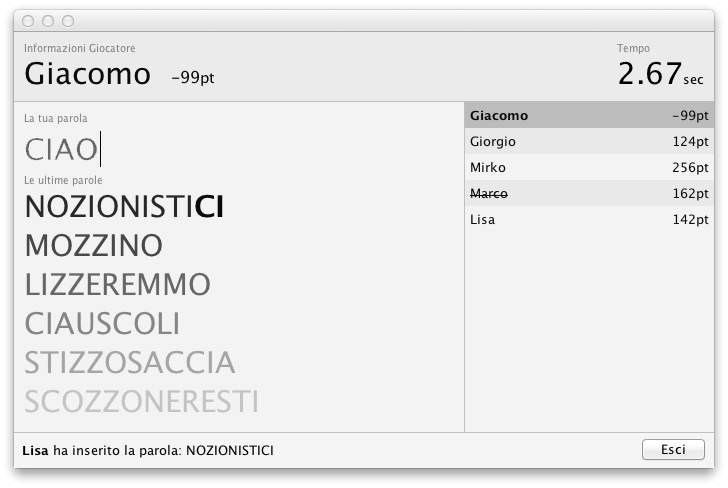
\includegraphics[scale=0.5]{imgs/screenshot.png}
		\caption{Una screenshot del gioco dove Giacomo detiene il turno e pertanto deve inserire una parola. Notare anche che Marco si è ritirato, oppure ha avuto un crash.}
	\end{center}
\end{figure}


\subsection{Regole del gioco}
All'inizio del gioco, i giocatori decidono di comune accordo una sequenza di gioco, ovvero l'ordine dei turni (giocando dal vivo, ci si mette spesso in cerchio). Ogni giocatore, al proprio turno, produrrà una singola parola. Il primo giocatore sceglie una parola qualunque, che deve essere \emph{presente nel dizionario} italiano utilizzato dal gioco. Dal secondo giocatore in poi, scatta la regola per la scelta della parola:

\begin{itemize}
\item Sia $w$ la parola prodotta dal giocatore precedente. Ad esempio ``VERIFICARE''.
\item Sia $w=w_1, w_2, \dots, w_n$ la sua suddivisione in sillabe. Ad esempio, ``VE'', ``RI'', ``FI'', ``CA'', ``RE''.
\item Sia $w'=w'_1, w'_2, \dots, w'_m$ la parola inserita dal giocatore corrente, e la sua suddivisione in sillabe.
\item La parola $w'$ è \emph{valida} se è presente nel dizionario e se $w_n = w'_1$, ovvero se la prima sillaba della nuova parola è uguale all'ultima sillaba della parola precedente. Ad esempio, ``REGINA'', ``RECITA'' e ``RETICOLO'' sono tutte parole valide, mentre ``RIONE'', ``RESPIRARE'', ``MANO'' sono tutte parole non valide.
\end{itemize}

Ciò quindi crea una sequenza di parole tutte collegate tra di essere per mezzo dell'ultima e della prima sillaba tra ogni coppia di parole. 

Per rendere più interessante il gioco, non basta che una parola sia \emph{valida} affinché si possano guadagnare dei punti per il proprio turno. Vi è un altro requisito fondamentale: la parola deve essere \emph{nuova}. Ovvero, la parola inserita non deve essere stata inserita precedentemente da alcun giocatore, durante il corso della corrente partita. Quindi, ogni giocatore deve tenere memoria della sequenza di parole generate da tutti i giocatori, ed evitare di riproporre una parola già inserita precedentemente. Per aiutare l'utente a capire le parole che sono state inserite, vengono visualizzate le ultime 6 parole.

Per complicare ulteriormente il gioco, e per evitare che il gioco duri troppo, ogni giocatore ha un limite di tempo entro il quale può proporre la sua parola.

Ogni giocatore, al proprio turno, può guadagnare o perdere punti, secondo le seguenti regole:
\begin{itemize}
\item Se la parola non è presente nel dizionario perde 80 punti.
\item Se la parola non è valida perde 80 punti.
\item Se la parola è \emph{valida}, ma non è \emph{nuova}, perde 100 punti.
\item Se il giocatore non è riuscito a produrre la parola entro il limite di tempo stabilito per un singolo turno, perde 60 punti.
\item Se la parola è valida e non è stata proposta precedentemente durante la stessa partita, il giocatore guadagna un numero di punti che dipende dalle lettere utilizzate (e.g. 1 punto per la lettera A, 8 per la lettera G), dalla lunghezza della parola (i.e. 5 punti in più per ogni lettera inserita dopo la quinta), e dai millesimi di secondo impiegati (i.e. 0.02 punti per ogni millisecondo che l'utente aveva ancora a disposizione per rispondere).
\end{itemize}

Da notare che, nel caso un giocatore abbia una perdita dei punti, la parola proposta non viene aggiunta alla lista delle parole utilizzate, il prossimo giocatore dovrà pertanto riprendere dalla parola dell'ultimo giocatore che era riuscito ad inserire una parola.

Un giocatore può ritirarsi in qualunque momento. In quel caso, il gioco continua tra i giocatori rimanenti, richiudendo il cerchio nella maniera naturale. Il gioco finisce quando un giocatore rimane da solo, oppure quando nessun giocatore riesce a produrre parole valide e nuove per un intero ciclo di gioco.

\subsection{Obiettivi del progetto}

L'obiettivo principale del presente progetto è la realizzazione del gioco in un ambiente distribuito, in cui varie entità distribuite (che chiameremo \emph{peer}, vista la loro intrinseca natura client/server) comunicano tra loro attraverso una rete asincrona, non affidabile, come quella di Internet. In questo tipo di contesto sono necessari coordinazione tra i peer, gestione di stati condivisi. [ ... FARE BENE STA PARTE, ED ELENCARE BENE I REQUISITI SCRITTI NEL SITO ].




\section{Aspetti progettuali}
% in cui si illustra il progetto svolto; in particolare si discutono i problemi specifici affrontati, le soluzioni valutate e proposte, e l'architettura astratta del sistema sviluppato.

\subsection{Interpretare RoundWord come un sistema distribuito}
Interpretare questo gioco nell'ambito dei sistemi distribuiti non è particolarmente difficile. Infatti, ogni giocatore controllato da un \emph{peer}, in una rete distribuita in stile peer-to-peer (senza overlay). I turni a ciclo suggeriscono l'idea di un protocollo in stile \emph{token-ring}, dove il detentore del turno viene equiparato al \emph{leader} attuale, e la leadership viene passata al prossimo peer allo scadere di ogni turno. Lo \emph{stato condiviso} tra i peer partecipanti consiste in:
\begin{itemize}
\item La lista dei peer attivi (non crashati)
\item La lista dei punteggi dei rispettivi giocatori
\item La lista completa delle parole inserite dai giocatori.
\item L'identità del detentore del turno attuale (ovvero del leader attuale)
\end{itemize}


\subsection{Architettura astratta}

Il sistema è composto di tre aree ben distinte: modello del gioco, controllori dei giocatori e comunicazione. La parte di modellazione del gioco si compone di tutte quelle classi che realizzano il gioco, senza prendere in considerazione il fatto che questo possa essere giocato in rete, e senza una concezione di interfaccia GUI. Tale modello ignora pertanto come i vari giocatori interagiscono, fornendo solamente dei metodi per cambiare lo stato del gioco, e generando eventi per segnalare tali cambiamenti. I controllori dei giocatori possono essere di tre tipi: un'interfaccia grafica che comunica con il giocatore reale permettendogli di poter giocare, un peer remoto che interagisce sfruttando la parte di comunicazione, o un giocatore automatico (principalmente utilizzato per debug, ma che comunque non si esclude possa essere utilizzato come un rimpiazzo per i giocatori che hanno subito un guasto).

La parte di comunicazione ha come incarico quello di interagire con gli altri peer presenti nel sistema, in modo da comunicare le parole che sono state inserite dal giocatore locale, e comunicare al modello del gioco quali sono quelle inserite dagli altri peer. Ogni peer ha pertanto il compito di gestire un particolare giocatore. Il peer utilizza due parti distinte che lo completano: una parte che funge da client (chiamata \emph{client side}) ed una parte che funge da server (chiamata \emph{server side}). 

...


\section{Aspetti implementativi}
% dettagli sulle scelte implementative, ed architettura specifica implementata. Inserire almeno il diagramma delle classi e uno delle interazioni secondo lo standard UML.

\subsection{Architettura}

\subsubsection{Modellazione del gioco}

Il gioco in sé viene rappresentato da poche classi: \texttt{GameTable}, \texttt{Word}, \texttt{Player} e \texttt{Dictionary}.

La classe \texttt{Word} rappresenta una parola del gioco. Consiste di una semplice stringa, ma ha numerosi metodi utili per scomporla in sillabe e determinarne il valore in punteggi. Inoltre essa è serializzabile, poiché deve poter essere inviata lungo la rete.  

La classe \texttt{Dictionary} rappresenta un dizionario, e contiene semplici metodi per il lookup di una parola.

La classe \texttt{Player} rappresenta un giocatore. Esso ha un nickname, un punteggio, uno stato (attivo o non attivo), ed altre informazioni necessarie per il gioco. Esso può essere controllato da un giocatore reale presente sullo stesso peer, da un agente che gioca automaticamente, oppure controllato un peer remoto.

La classe \texttt{GameTable} rappresenta il tavolo di gioco. Essa contiene informazioni quali: la lista delle parole che sono state inserite, come anche la lista dei giocatori, ed il giocatore che detiene il turno. Inoltre ha dei metodi per modificare lo stato del gioco, come quello per determinare chi è il prossimo detentore del turno, o per inserire una nuova parola. Tale classe non ha un'idea del fatto di come viene controllato un giocatore; seguendo il design pattern chiamato \textit{Observer Pattern}, la classe è stata progettata per generare degli eventi, quali ad esempio l'inserimento di una nuova parola, il cambio del turno, o la terminazione del gioco. Sono poi presenti diversi listener che rispondono in maniera passiva a questi eventi seguendo delle azioni opportune. Questi stessi listener possono comunque avere dei ruoli attivi, come ad esempio l'inserimento di nuove parole. 

L'entità più semplice, chiamata \texttt{FakePlayer}, che rappresenta un agente che gioca automaticamente, consiste ad esempio in un semplice loop, che inserisce una parola, e che rimane in attesa fin tanto che il \texttt{GameTable} non genera un evento, in modo da segnalare che tale agente è il detentore del prossimo turno. 

Al contrario, un giocatore reale ha tanti oggetti, che rappresentano varie componenti dell'interfaccia. Ognuno di essi può fungere anche da listener, in modo da poter aggiornare le varie informazioni che gli competono. Inoltre, l'interfaccia ha anche un ruolo attivo, poiché inserisce le parole che sono state scritte dall'utente, calcolando anche il tempo impiegato per farlo.

Più complicato è invece un giocatore controllato da un peer remoto. Il \texttt{Peer}, che funge anche da listener, può reagire ad un evento, quale ad esempio l'inserimento di una nuova parola, mandando dei messaggi per informare anche agli altri peer di tale evento. Può poi inserire nuove parole sulla base dei messaggi ricevuti dagli altri peer, cambiare lo stato di un giocatore (ad esempio a causa di un crash), oppure decidere chi possederà il prossimo turno in base sullo stato degli altri peer.

\begin{figure}
	\begin{center}
		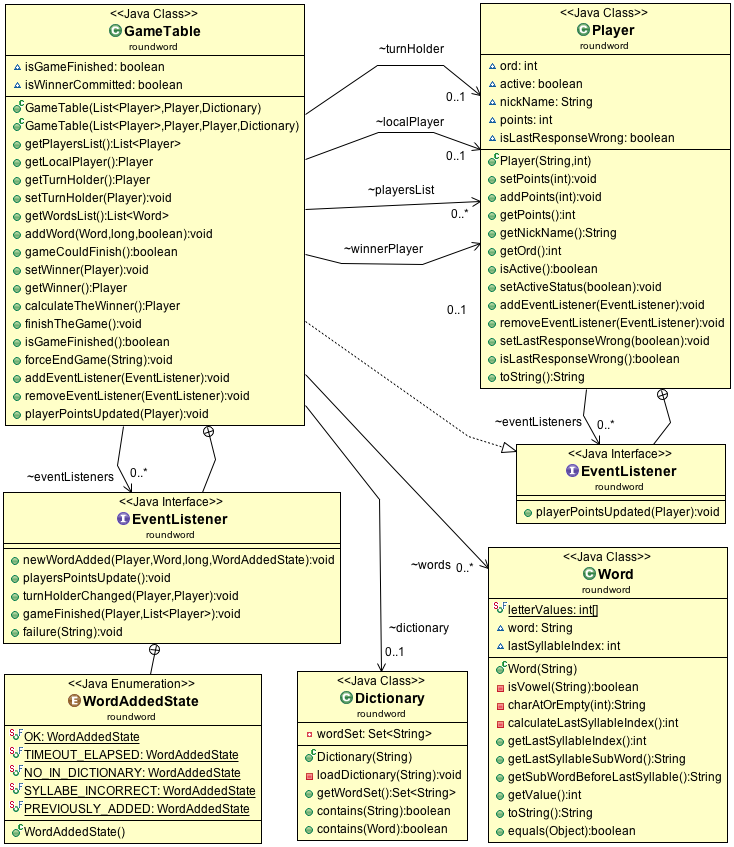
\includegraphics[scale=0.5]{imgs/ClassDiagram1.png}
		\caption{}
	\end{center}
\end{figure}

\subsubsection{Comunicazione}

Descrizione peer, clientside, serverside, ecc...

\begin{figure}
	\begin{center}
		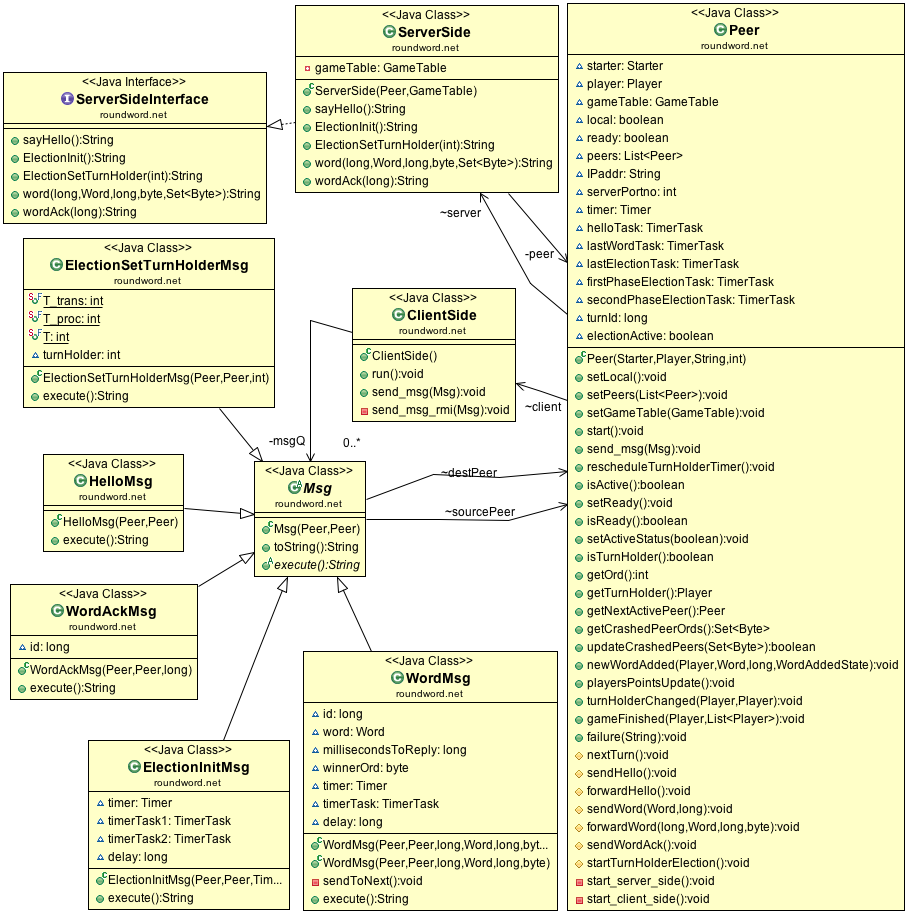
\includegraphics[scale=0.4]{imgs/ClassDiagram2.png}
		\caption{}
	\end{center}
\end{figure}



\section{Valutazione}
% confronto delle soluzioni proposte con soluzioni analoghe allo stato dell'arte.

TODO: Dizionari divisi per sezioni, ad esempio tutte le parole che riguardano l'automobilismo. Si potrebbe ampliare il gioco in modo da restringere le parole che possono essere utilizzate a quelle che appartengono solamente ad una determinata categoria.

TODO: altri casi di terminazione, basati ad esempio sul fatto che un giocatore vince se doppia i punti degli altri ecc

TODO: rimpiazzi giocatori falliti


\section{Conclusioni}
% commenti conclusivi su possibili miglioramenti di quanto discusso, e possibili linee di intervento futuro.




% Bibliography
\bibliographystyle{ACM-Reference-Format-Journals}
\bibliography{riferimenti}


\end{document}
% End of v2-acmlarge-sample.tex (March 2012) - Gerry Murray, ACM
